\documentclass[9pt,aspectratio=169]{beamer}

\usetheme{Madrid}
\definecolor{madridgreen}{RGB}{0,110,60}
\usecolortheme[named=madridgreen]{structure}
\setbeamertemplate{navigation symbols}{}

\usepackage{amsmath,amssymb}
\usepackage{booktabs}
\usepackage{array}
\usepackage{tikz}
% Shared colours, TikZ styles and figure macros.
% Used by delay_attacks_beamer.tex (the slides) and figures.tex (PNG export for the PowerPoint).

\definecolor{madridgreen}{RGB}{0,110,60}
\definecolor{hitgreen}{RGB}{46,160,90}
\definecolor{missred}{RGB}{200,40,40}
\definecolor{softgreen}{RGB}{228,242,233}
\definecolor{softred}{RGB}{250,228,228}
\definecolor{inkgray}{RGB}{90,90,90}

\usetikzlibrary{arrows.meta,positioning,calc,shapes.geometric,shapes.symbols,decorations.pathreplacing}

\tikzset{
  blk/.style={draw=madridgreen,very thick,rounded corners=3pt,fill=softgreen,minimum height=8mm,align=center,font=\small},
  arr/.style={-{Stealth[length=2.2mm]},very thick,draw=inkgray},
  hit/.style={draw=hitgreen!70!black,fill=hitgreen!80,minimum width=6mm,minimum height=5mm},
  miss/.style={draw=missred!70!black,fill=missred!85,minimum width=6mm,minimum height=5mm},
}

% ---------------------------------------------------------------- control loop
\newcommand{\FigLoop}{%
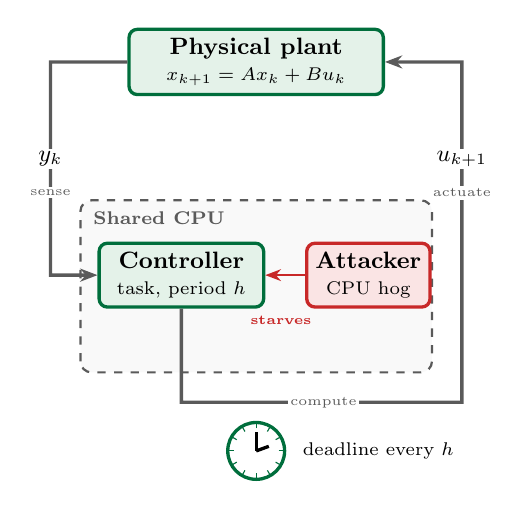
\begin{tikzpicture}[scale=0.95,transform shape]
  \node[blk,minimum width=3.4cm] (plant) at (0,2.6) {\textbf{Physical plant}\\[-1pt]{\scriptsize $x_{k+1}=Ax_k+Bu_k$}};
  \draw[dashed,thick,draw=inkgray,rounded corners=4pt,fill=gray!5] (-2.35,-1.55) rectangle (2.35,0.75);
  \node[font=\scriptsize\bfseries,text=inkgray,anchor=north west] at (-2.3,0.72) {Shared CPU};
  \node[blk,minimum width=2.2cm] (ctrl) at (-1.0,-0.25) {\textbf{Controller}\\[-1pt]{\scriptsize task, period $h$}};
  \node[draw=missred,very thick,rounded corners=3pt,fill=softred,align=center,font=\small,minimum height=8mm] (att) at (1.5,-0.25) {\textbf{Attacker}\\[-1pt]{\scriptsize CPU hog}};
  \draw[-{Stealth[length=2mm]},thick,missred] (att.west) -- (ctrl.east);
  \node[font=\tiny\bfseries,text=missred] at (0.33,-0.85) {starves};
  \draw[arr] (plant.west) -| (-2.75,-0.25) -- (ctrl.west);
  \node[font=\small,fill=white,inner sep=1pt] at (-2.75,1.3) {$y_k$};
  \node[font=\tiny,text=inkgray,fill=white,inner sep=1pt] at (-2.75,0.85) {sense};
  \draw[arr] (ctrl.south) |- (2.75,-1.95) -- (2.75,2.6) -- (plant.east);
  \node[font=\small,fill=white,inner sep=1pt] at (2.75,1.3) {$u_{k+1}$};
  \node[font=\tiny,text=inkgray,fill=white,inner sep=1pt] at (2.75,0.85) {actuate};
  \node[font=\tiny,text=inkgray,fill=white,inner sep=1pt] at (0.9,-1.95) {compute};
  \begin{scope}[shift={(0,-2.6)}]
    \draw[very thick,madridgreen,fill=white] (0,0) circle (0.38);
    \foreach \a in {0,30,...,330} \draw[madridgreen] (\a:0.30) -- (\a:0.36);
    \draw[very thick] (0,0) -- (90:0.25);
    \draw[very thick] (0,0) -- (20:0.18);
    \node[right=4mm,font=\scriptsize,align=left] at (0.1,0) {deadline every $h$};
  \end{scope}
\end{tikzpicture}}

% ---------------------------------------------------------------- taxonomy
\newcommand{\FigTaxonomy}{%
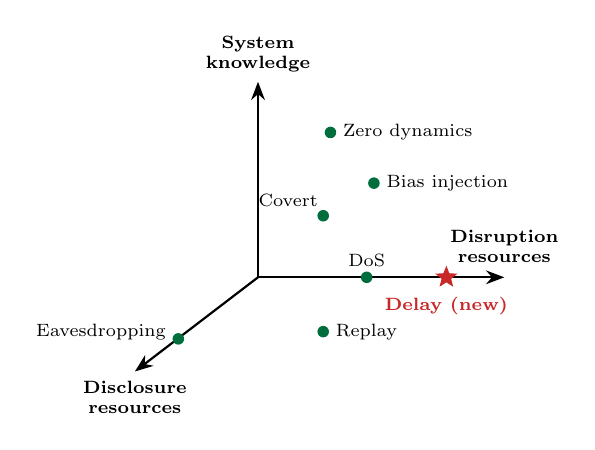
\begin{tikzpicture}[scale=0.92,transform shape,
  pt/.style={circle,fill=madridgreen,inner sep=1.6pt},
  lb/.style={font=\scriptsize}]
  \draw[-{Stealth},thick] (0,0) -- (0,2.7) node[above,font=\scriptsize\bfseries,align=center]{System\\knowledge};
  \draw[-{Stealth},thick] (0,0) -- (3.4,0) node[above,font=\scriptsize\bfseries,align=center,yshift=2pt]{Disruption\\resources};
  \draw[-{Stealth},thick] (0,0) -- (-1.7,-1.3) node[below,font=\scriptsize\bfseries,align=center]{Disclosure\\resources};
  \node[pt] at (-1.1,-0.85) {}; \node[lb,left] at (-1.15,-0.75) {Eavesdropping};
  \node[pt] at (1.5,0) {}; \node[lb,above] at (1.5,0.02) {DoS};
  \node[pt] at (0.9,-0.75) {}; \node[lb,right] at (0.95,-0.75) {Replay};
  \node[pt] at (1.6,1.3) {}; \node[lb,right] at (1.65,1.3) {Bias injection};
  \node[pt] at (1.0,2.0) {}; \node[lb,right] at (1.05,2.0) {Zero dynamics};
  \node[pt] at (0.9,0.85) {}; \node[lb,above left] at (0.95,0.85) {Covert};
  \node[star,star points=5,star point ratio=2.3,fill=missred,inner sep=1.4pt] at (2.6,0) {};
  \node[font=\scriptsize\bfseries,text=missred,below] at (2.6,-0.15) {Delay (new)};
\end{tikzpicture}}

% ---------------------------------------------------------------- attack timeline with hold / zero
\newcommand{\FigTimeline}{%
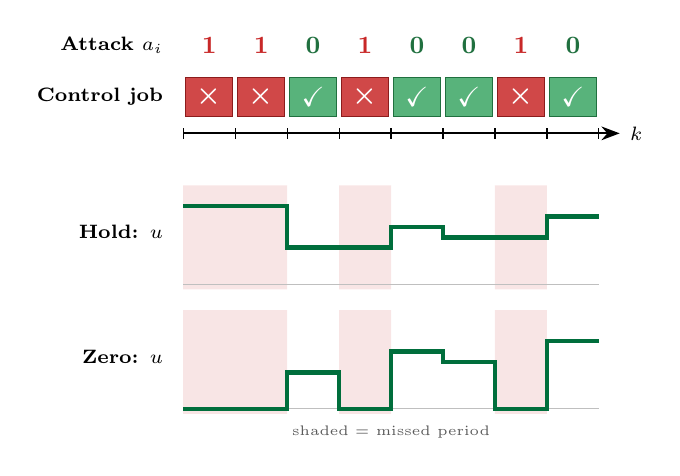
\begin{tikzpicture}[x=6.6mm,y=6.6mm]
  \node[font=\scriptsize\bfseries,anchor=east] at (-0.2,1.5) {Attack $a_i$};
  \node[font=\scriptsize\bfseries,anchor=east] at (-0.2,0.5) {Control job};
  \foreach \b [count=\i from 0] in {1,1,0,1,0,0,1,0} {
    \ifnum\b=1
      \node[font=\small\bfseries,text=missred] at (\i+0.5,1.5) {1};
      \node[miss] at (\i+0.5,0.5) {\textcolor{white}{\boldmath$\times$}};
    \else
      \node[font=\small\bfseries,text=hitgreen!70!black] at (\i+0.5,1.5) {0};
      \node[hit] at (\i+0.5,0.5) {\textcolor{white}{\checkmark}};
    \fi
  }
  \draw[-{Stealth},thick] (0,-0.2) -- (8.4,-0.2) node[right,font=\scriptsize]{$k$};
  \foreach \i in {0,...,8} \draw (\i,-0.3) -- (\i,-0.1);
  \begin{scope}[shift={(0,-3.1)}]
    \node[font=\scriptsize\bfseries,anchor=east] at (-0.2,1.0) {Hold: $u$};
    \fill[missred,opacity=0.12] (0,-0.1) rectangle (2,1.9) (3,-0.1) rectangle (4,1.9) (6,-0.1) rectangle (7,1.9);
    \draw[gray!50] (0,0) -- (8,0);
    \draw[ultra thick,madridgreen] (0,1.5) -- (2,1.5) -- (2,0.7) -- (4,0.7) -- (4,1.1) -- (5,1.1) -- (5,0.9) -- (7,0.9) -- (7,1.3) -- (8,1.3);
  \end{scope}
  \begin{scope}[shift={(0,-5.5)}]
    \node[font=\scriptsize\bfseries,anchor=east] at (-0.2,1.0) {Zero: $u$};
    \fill[missred,opacity=0.12] (0,-0.1) rectangle (2,1.9) (3,-0.1) rectangle (4,1.9) (6,-0.1) rectangle (7,1.9);
    \draw[gray!50] (0,0) -- (8,0);
    \draw[ultra thick,madridgreen] (0,0) -- (2,0) -- (2,0.7) -- (3,0.7) -- (3,0) -- (4,0) -- (4,1.1) -- (5,1.1) -- (5,0.9) -- (6,0.9) -- (6,0) -- (7,0) -- (7,1.3) -- (8,1.3);
    \node[font=\tiny,text=inkgray,anchor=north] at (4,-0.15) {shaded = missed period};
  \end{scope}
\end{tikzpicture}}

% ---------------------------------------------------------------- the three detector pictures
\newcommand{\FigWatchdog}{%
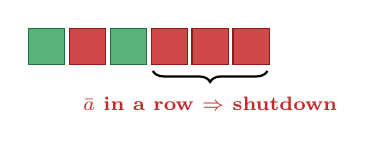
\begin{tikzpicture}[x=5.2mm,y=5.2mm]
  \foreach \b [count=\i from 0] in {0,1,0,1,1,1} {
    \ifnum\b=1 \node[miss,minimum width=4.6mm,minimum height=4.6mm] at (\i,0) {};
    \else \node[hit,minimum width=4.6mm,minimum height=4.6mm] at (\i,0) {}; \fi }
  \draw[decorate,decoration={brace,amplitude=4pt,mirror},thick] (2.6,-0.6) -- (5.4,-0.6);
  \node[font=\scriptsize\bfseries,text=missred] at (4,-1.4) {$\bar a$ in a row $\Rightarrow$ shutdown};
\end{tikzpicture}}

\newcommand{\FigWindow}{%
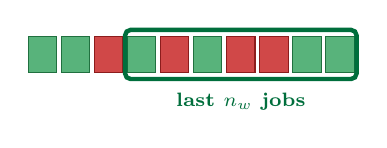
\begin{tikzpicture}[x=4.2mm,y=5.2mm]
  \foreach \b [count=\i from 0] in {0,0,1,0,1,0,1,1,0,0} {
    \ifnum\b=1 \node[miss,minimum width=3.6mm,minimum height=4.6mm] at (\i,0) {};
    \else \node[hit,minimum width=3.6mm,minimum height=4.6mm] at (\i,0) {}; \fi }
  \draw[madridgreen,ultra thick,rounded corners=2pt] (2.5,-0.6) rectangle (9.5,0.6);
  \node[font=\scriptsize\bfseries,text=madridgreen] at (6,-1.15) {last $n_w$ jobs};
\end{tikzpicture}}

\newcommand{\FigHistogram}{%
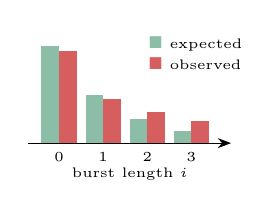
\begin{tikzpicture}[x=5.6mm,y=5.6mm]
  \draw[-{Stealth}] (-0.3,0) -- (4.3,0);
  \foreach \i/\e/\o in {0/2.2/2.1,1/1.1/1.0,2/0.55/0.7,3/0.28/0.5} {
    \fill[madridgreen!45] (\i,0) rectangle (\i+0.4,\e);
    \fill[missred!75] (\i+0.4,0) rectangle (\i+0.8,\o);
    \node[font=\tiny,below] at (\i+0.4,0) {\i};
  }
  \node[font=\tiny,anchor=north] at (2,-0.35) {burst length $i$};
  \node[font=\tiny,anchor=west] at (2.2,2.25) {\textcolor{madridgreen!45}{$\blacksquare$} expected};
  \node[font=\tiny,anchor=west] at (2.2,1.8) {\textcolor{missred!75}{$\blacksquare$} observed};
\end{tikzpicture}}

% ---------------------------------------------------------------- five-step icons (each about 1.6 x 1.1 cm)
\newcommand{\IconSetting}{%
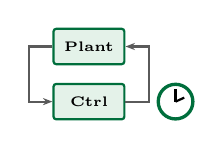
\begin{tikzpicture}[x=1mm,y=1mm]
  \node[draw=madridgreen,thick,fill=softgreen,rounded corners=1pt,minimum width=9mm,minimum height=4.5mm,font=\tiny\bfseries] (p) at (0,6) {Plant};
  \node[draw=madridgreen,thick,fill=softgreen,rounded corners=1pt,minimum width=9mm,minimum height=4.5mm,font=\tiny\bfseries] (c) at (0,-1) {Ctrl};
  \draw[-{Stealth[length=1.2mm]},thick,inkgray] (p.west) -- ++(-3,0) |- (c.west);
  \draw[-{Stealth[length=1.2mm]},thick,inkgray] (c.east) -- ++(3,0) |- (p.east);
  \draw[very thick,madridgreen,fill=white] (11,-1) circle (2.2);
  \draw[thick] (11,-1) -- (11,0.6); \draw[thick] (11,-1) -- (12.1,-0.5);
\end{tikzpicture}}

\newcommand{\IconAttack}{%
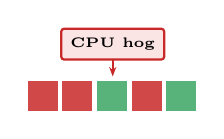
\begin{tikzpicture}[x=1mm,y=1mm]
  \foreach \b [count=\i from 0] in {1,1,0,1,0} {
    \ifnum\b=1 \fill[missred!85] (\i*4.4,0) rectangle ++(3.8,3.8);
    \else \fill[hitgreen!80] (\i*4.4,0) rectangle ++(3.8,3.8); \fi }
  \node[draw=missred,thick,fill=softred,rounded corners=1pt,font=\tiny\bfseries,minimum width=12mm] at (10.8,8.5) {CPU hog};
  \draw[-{Stealth[length=1.2mm]},thick,missred] (10.8,6.6) -- (10.8,4.4);
\end{tikzpicture}}

\newcommand{\IconDetector}{%
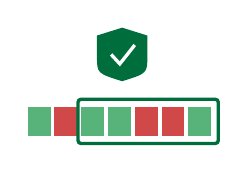
\begin{tikzpicture}[x=1mm,y=1mm]
  \foreach \b [count=\i from 0] in {0,1,0,0,1,1,0} {
    \ifnum\b=1 \fill[missred!85] (\i*3.4,0) rectangle ++(2.9,3.6);
    \else \fill[hitgreen!80] (\i*3.4,0) rectangle ++(2.9,3.6); \fi }
  \draw[madridgreen,very thick,rounded corners=1pt] (6.4,-1) rectangle (24.2,4.6);
  \begin{scope}[shift={(12,10.5)}]
    \fill[madridgreen] (0,3.2) -- (3.2,2.2) -- (3.2,-0.4) .. controls (3.2,-2.6) .. (0,-3.6) .. controls (-3.2,-2.6) .. (-3.2,-0.4) -- (-3.2,2.2) -- cycle;
    \draw[white,very thick] (-1.4,-0.2) -- (-0.3,-1.4) -- (1.6,1.0);
  \end{scope}
\end{tikzpicture}}

\newcommand{\IconOptimise}{%
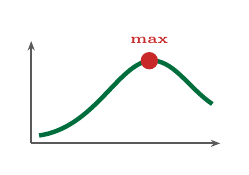
\begin{tikzpicture}[x=1mm,y=1mm]
  \draw[-{Stealth[length=1.2mm]},thick,inkgray] (0,0) -- (24,0);
  \draw[-{Stealth[length=1.2mm]},thick,inkgray] (0,0) -- (0,13);
  \draw[ultra thick,madridgreen] (1,1) .. controls (8,2) and (11,10) .. (15,10.5) .. controls (18,10.8) and (20,7) .. (23,5);
  \fill[missred] (15,10.5) circle (1.1);
  \node[font=\tiny\bfseries,text=missred,anchor=south] at (15,11.5) {max};
\end{tikzpicture}}

\newcommand{\IconPlants}{%
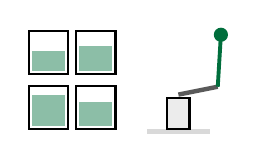
\begin{tikzpicture}[x=1mm,y=1mm]
  \foreach \x/\y/\h in {0/7/2.5,6/7/3.2,0/0/4,6/0/3} {
    \draw[thick] (\x,\y) rectangle ++(5,5.5);
    \fill[madridgreen!45] (\x+0.4,\y+0.4) rectangle ++(4.2,\h);
  }
  \begin{scope}[shift={(19,0)}]
    \fill[gray!30] (-4,-0.6) rectangle (4,0);
    \draw[thick,fill=gray!15] (-1.4,0) rectangle (1.4,4);
    \draw[line width=1.6pt,inkgray] (0,4.4) -- (5,5.4);
    \draw[line width=1.4pt,madridgreen] (5,5.4) -- (5.4,12);
    \fill[madridgreen] (5.4,12) circle (0.9);
  \end{scope}
\end{tikzpicture}}

% ---------------------------------------------------------------- the two test plants
\newcommand{\FigTank}{%
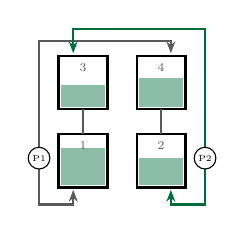
\begin{tikzpicture}[x=1cm,y=1cm,scale=0.62,transform shape]
  \foreach \x/\y/\h/\n in {0/1.6/0.5/3,1.6/1.6/0.65/4,0/0/0.8/1,1.6/0/0.6/2} {
    \draw[thick,fill=white] (\x,\y) rectangle (\x+1,\y+1.1);
    \fill[madridgreen!45] (\x+0.05,\y+0.05) rectangle (\x+0.95,\y+\h);
    \node[font=\scriptsize,text=inkgray] at (\x+0.5,\y+0.85) {\n};
  }
  \draw[thick,inkgray] (0.5,1.6) -- (0.5,1.1);
  \draw[thick,inkgray] (2.1,1.6) -- (2.1,1.1);
  \draw[thick,inkgray,-{Stealth[length=1.5mm]}] (-0.4,0.6) -- (-0.4,3.0) -- (2.3,3.0) -- (2.3,2.75);
  \draw[thick,inkgray,-{Stealth[length=1.5mm]}] (-0.4,0.6) -- (-0.4,-0.35) -- (0.3,-0.35) -- (0.3,-0.05);
  \draw[thick,madridgreen,-{Stealth[length=1.5mm]}] (3.0,0.6) -- (3.0,3.25) -- (0.3,3.25) -- (0.3,2.75);
  \draw[thick,madridgreen,-{Stealth[length=1.5mm]}] (3.0,0.6) -- (3.0,-0.35) -- (2.3,-0.35) -- (2.3,-0.05);
  \node[draw,circle,fill=white,inner sep=1.5pt,font=\tiny] at (-0.4,0.6) {P1};
  \node[draw,circle,fill=white,inner sep=1.5pt,font=\tiny] at (3.0,0.6) {P2};
\end{tikzpicture}}

\newcommand{\FigFuruta}{%
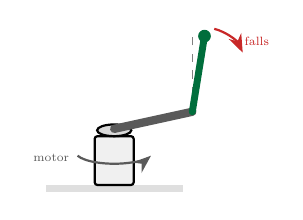
\begin{tikzpicture}[x=1cm,y=1cm,scale=0.62,transform shape]
  \fill[gray!25] (-1.4,-0.15) rectangle (1.4,0);
  \draw[thick,fill=gray!12,rounded corners=1pt] (-0.4,0) rectangle (0.4,1.0);
  \draw[thick,fill=gray!30] (0,1.12) ellipse (0.35 and 0.12);
  \draw[line width=3pt,inkgray,line cap=round] (0,1.15) -- (1.6,1.5);
  \draw[dashed,gray] (1.6,1.5) -- (1.6,3.2);
  \draw[line width=2.5pt,madridgreen,line cap=round] (1.6,1.5) -- (1.85,3.05);
  \fill[madridgreen] (1.85,3.05) circle (0.13);
  \draw[-{Stealth},thick,missred] (2.05,3.2) arc (75:25:0.9);
  \node[font=\scriptsize,text=missred,anchor=west] at (2.55,2.95) {falls};
  \draw[-{Stealth},thick,inkgray] (-0.75,0.6) arc (200:340:0.8 and 0.25);
  \node[font=\scriptsize,text=inkgray,anchor=east] at (-0.8,0.55) {motor};
\end{tikzpicture}}

% ---------------------------------------------------------------- defences watch the data, not the clock
\newcommand{\FigBlindSpot}{%
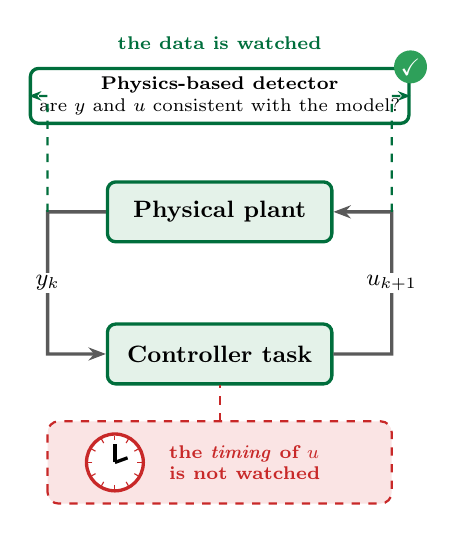
\begin{tikzpicture}[scale=0.95,transform shape]
  \node[blk,minimum width=3.0cm] (plant) at (0,1.9) {\textbf{Physical plant}};
  \node[blk,minimum width=3.0cm] (ctrl) at (0,0) {\textbf{Controller task}};
  \draw[arr] (plant.west) -- (-2.3,1.9) -- (-2.3,0) -- (ctrl.west);
  \draw[arr] (ctrl.east) -- (2.3,0) -- (2.3,1.9) -- (plant.east);
  \node[font=\small,fill=white,inner sep=1pt] at (-2.3,0.95) {$y_k$};
  \node[font=\small,fill=white,inner sep=1pt] at (2.3,0.95) {$u_{k+1}$};
  % physics-based detector watching the data
  \node[draw=madridgreen,very thick,rounded corners=3pt,fill=white,align=center,font=\scriptsize,minimum width=3.4cm] (det) at (0,3.45)
     {\textbf{Physics-based detector}\\ are $y$ and $u$ consistent with the model?};
  \draw[dashed,thick,madridgreen,-{Stealth[length=1.6mm]}] (-2.3,1.9) -- (-2.3,3.45) -- (det.west);
  \draw[dashed,thick,madridgreen,-{Stealth[length=1.6mm]}] (2.3,1.9) -- (2.3,3.45) -- (det.east);
  \node[circle,fill=hitgreen,text=white,font=\small\bfseries,inner sep=1pt] at (det.north east) {\checkmark};
  \node[font=\scriptsize\bfseries,text=madridgreen,anchor=south] at (0,3.95) {the data is watched};
  % the unwatched clock
  \begin{scope}[shift={(0,-1.45)}]
    \draw[dashed,thick,missred,rounded corners=4pt,fill=softred] (-2.3,-0.55) rectangle (2.3,0.55);
    \draw[very thick,missred,fill=white] (-1.4,0) circle (0.38);
    \foreach \a in {0,30,...,330} \draw[missred,shift={(-1.4,0)}] (\a:0.30) -- (\a:0.36);
    \draw[very thick,shift={(-1.4,0)}] (0,0) -- (90:0.25);
    \draw[very thick,shift={(-1.4,0)}] (0,0) -- (20:0.18);
    \node[font=\scriptsize\bfseries,text=missred,align=left,anchor=west] at (-0.8,0) {the \emph{timing} of $u$\\ is not watched};
  \end{scope}
  \draw[dashed,thick,missred] (0,-0.9) -- (ctrl.south);
\end{tikzpicture}}


% Footer: source line, then one green bar with the title and the page number (no presenter, no date).
\setbeamertemplate{footline}{%
  \leavevmode\hspace*{1.2em}{\fontsize{5}{6}\selectfont\color{inkgray}Source: T.~Nauta, H.~Sandberg and M.~Maggio, ``Stealthy Computational Delay Attacks on Control Systems,'' ICCPS 2025. DOI 10.1145/3716550.3722013}\par\vspace{2pt}%
  \begin{beamercolorbox}[wd=\paperwidth,ht=2.4ex,dp=1ex]{title in head/foot}%
    \usebeamerfont{title in head/foot}\hspace*{2ex}\hfill\insertshorttitle\hfill\insertframenumber{} / \inserttotalframenumber\hspace*{2ex}%
  \end{beamercolorbox}}

\newcommand{\takeaway}[3]{%
  \noindent\begin{minipage}[t]{0.085\linewidth}\vspace{0pt}%
    \tikz\node[circle,fill=madridgreen,text=white,font=\small\bfseries,minimum size=5.5mm,inner sep=0pt]{#1};%
  \end{minipage}\hfill
  \begin{minipage}[t]{0.895\linewidth}\vspace{0pt}\raggedright
    {\color{madridgreen}\textbf{#2}}\\[0.1em]{\small #3}%
  \end{minipage}\par\vspace{0.75em}}

% One card of the "paper in five steps" slide: number, icon, title, section, text
\newcommand{\stepcard}[5]{%
  \begin{tikzpicture}
    \node[draw=madridgreen,thick,rounded corners=3pt,fill=white,minimum width=2.62cm,minimum height=4.3cm,anchor=north] (c) at (0,0) {};
    \fill[softgreen,rounded corners=3pt] ([xshift=0.6pt,yshift=-0.6pt]c.north west) rectangle ([xshift=-0.6pt,yshift=-1.75cm]c.north east);
    \node[circle,fill=madridgreen,text=white,font=\small\bfseries,inner sep=0pt,minimum size=5mm,draw=white,thick] at (c.north) {#1};
    \node at (0,-0.95) {\scalebox{0.9}{#2}};
    \node[anchor=north,font=\small\bfseries,text=madridgreen] at (0,-1.85) {#3};
    \node[anchor=north,font=\tiny,text=inkgray] at (0,-2.22) {#4};
    \node[anchor=north,text width=2.4cm,align=center,font=\footnotesize,execute at begin node={\hyphenpenalty=10000\relax}] at (0,-2.52) {#5};
  \end{tikzpicture}}

\title[Stealthy Computational Delay Attacks on Control Systems]{Stealthy Computational Delay Attacks\\ on Control Systems}
\subtitle{Talitha Nauta, Henrik Sandberg and Martina Maggio \quad$\cdot$\quad ACM/IEEE ICCPS 2025}
\date{}

\begin{document}

%===================================================================
\begin{frame}[plain]
\vspace*{1.2em}
\begin{beamercolorbox}[sep=10pt,center,rounded=true,shadow=true]{title}
  {\usebeamerfont{title}\inserttitle\par}
  \vspace{0.5em}
  {\usebeamerfont{subtitle}\small\insertsubtitle\par}
\end{beamercolorbox}
\vspace{1.6em}
\begin{center}
  {\scriptsize\color{inkgray}\textsc{Presented by}}\\[0.6em]
  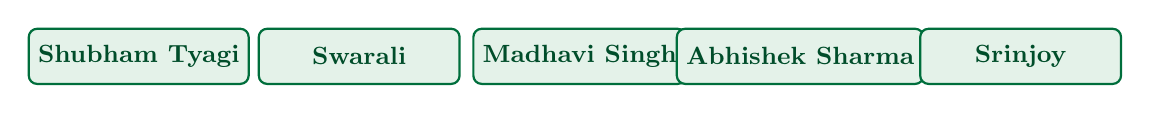
\begin{tikzpicture}
    \foreach \n [count=\i from 0] in {Shubham Tyagi,Swarali,Madhavi Singh,Abhishek Sharma,Srinjoy} {
      \node[draw=madridgreen,thick,rounded corners=3pt,fill=softgreen,font=\small\bfseries,text=madridgreen!70!black,minimum width=2.55cm,minimum height=7mm] at (\i*2.8,0) {\n};
    }
  \end{tikzpicture}\\[1.6em]
  {\small Embedded and Cyber-Physical Systems}
\end{center}
\end{frame}

%===================================================================
\begin{frame}{Presentation Roadmap}
\centering
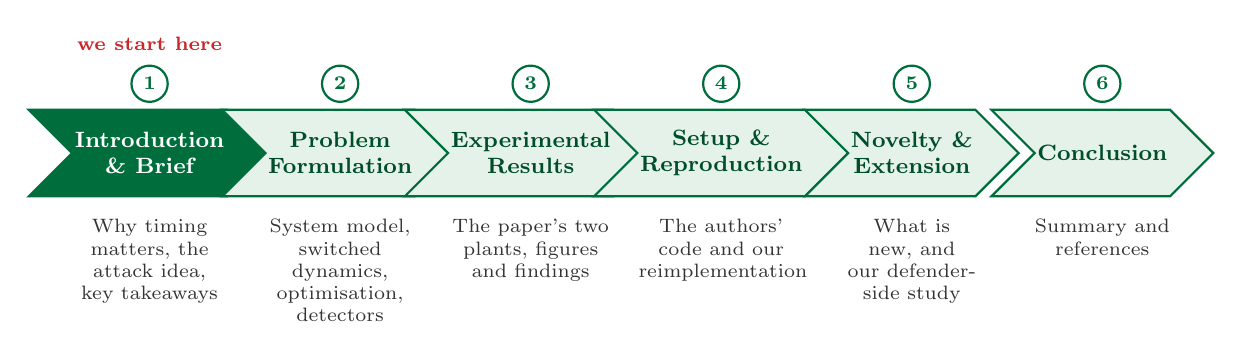
\begin{tikzpicture}[
  chev/.style={signal,signal to=east,signal from=west,minimum width=2.35cm,minimum height=1.1cm,
               draw=madridgreen,thick,fill=softgreen,text=madridgreen!70!black,font=\footnotesize\bfseries,align=center,inner sep=1pt},
  first/.style={chev,fill=madridgreen,text=white,draw=madridgreen},
  desc/.style={text width=2.1cm,align=center,execute at begin node={\hyphenpenalty=10000\relax},font=\scriptsize,text=black!80,anchor=north}]
  \foreach \t/\d [count=\i] in {
    {Introduction\\\& Brief}/{Why timing matters, the attack idea, key takeaways},
    {Problem\\Formulation}/{System model, switched dynamics, optimisation, detectors},
    {Experimental\\Results}/{The paper's two plants, figures and findings},
    {Setup \&\\Reproduction}/{The authors' code and our reimplementation},
    {Novelty \&\\Extension}/{What is new, and our defender-side study},
    {Conclusion}/{Summary and references}} {
    \pgfmathsetmacro{\x}{(\i-1)*2.42}
    \ifnum\i=1 \node[first] (c\i) at (\x,0) {\t}; \else \node[chev] (c\i) at (\x,0) {\t}; \fi
    \node[circle,fill=white,draw=madridgreen,thick,font=\scriptsize\bfseries,text=madridgreen,inner sep=0pt,minimum size=4.6mm] at (\x,0.88) {\i};
    \node[desc] at (\x,-0.72) {\d};
  }
  \node[font=\scriptsize\bfseries,text=missred,anchor=south] at (0,1.18) {we start here};
\end{tikzpicture}

\vspace{1.5em}
\begin{block}{How the parts connect}
We go from the \textbf{idea} (part 1) to the \textbf{model} (part 2), then to the \textbf{evidence} (parts 3 and 4), and finish with \textbf{our own contribution} (part 5).
\end{block}
\end{frame}

%===================================================================
\begin{frame}{Introduction: Why Timing Is a Security Problem}
\begin{columns}[T]
\begin{column}{0.50\textwidth}
\begin{itemize}\setlength\itemsep{0.4em}
  \item A \textbf{cyber-physical system} couples computation with a physical process: power grids, factories, vehicles, medical devices.
  \item Its controller is a \textbf{periodic task} that must deliver a new command before every \textbf{deadline}.
  \item Famous attacks such as \textbf{Stuxnet (2010)} and the \textbf{German steel mill (2014)} forged the \emph{data}: sensor readings or commands.
  \item So defences learned to check the data. \textbf{Physics-based detectors} ask whether $y$ and $u$ agree with the plant model.
\end{itemize}
\vspace{0.3em}
\begin{alertblock}{The blind spot}
A delay forges nothing, so the loop still obeys its model. What if an attacker only changes \emph{when} the command arrives?
\end{alertblock}
\end{column}
\begin{column}{0.48\textwidth}
\centering
\FigBlindSpot
\end{column}
\end{columns}
\end{frame}

%===================================================================
\begin{frame}{Introduction: Where Delay Attacks Fit}
\begin{columns}[T]
\begin{column}{0.40\textwidth}
\centering
{\small\textbf{Taxonomy of CPS attacks} {\scriptsize (Teixeira et al.)}}\\[0.3em]
\FigTaxonomy\\[0.2em]
{\scriptsize The paper adds the \textcolor{missred}{\textbf{delay attack}}: it needs only disruption resources, no access to the data.}
\end{column}
\begin{column}{0.58\textwidth}
\renewcommand{\arraystretch}{1.35}
{\footnotesize
\begin{tabular}{>{\raggedright\arraybackslash\bfseries}p{2.0cm}>{\raggedright\arraybackslash}p{1.65cm}>{\raggedright\arraybackslash}p{1.45cm}>{\raggedright\arraybackslash}p{2.0cm}}
\toprule
 & \textbf{False data injection} & \textbf{Denial of service} & \textcolor{missred}{\textbf{Computational delay}}\\
\midrule
What it changes & sensor or actuator values & availability & \emph{timing} of the control job\\
Needs to read data? & yes & no & \textbf{no}\\
How it looks & model mismatch & large and obvious & like normal timing jitter\\
Physics detector catches it? & often & yes & \textbf{no}: $y$ and $u$ stay consistent\\
\bottomrule
\end{tabular}}

\vspace{0.6em}
\begin{block}{Why it is hard to spot}
Industrial controllers already miss deadlines now and then in normal operation. A few extra, well-placed misses look exactly like that background noise.
\end{block}
\end{column}
\end{columns}
\end{frame}

%===================================================================
\begin{frame}{Brief of the Paper: The Attack Idea}
\begin{itemize}
  \item \textbf{CPU starvation:} when a control job starts, the attacker runs a task that holds the processor, so the job misses its deadline.
  \item Each period the attacker decides: \textcolor{hitgreen!80!black}{\textbf{0 = let it run}}, \textcolor{missred}{\textbf{1 = force a miss}}.
\end{itemize}
\vspace{0.2em}
\begin{columns}[T]
\begin{column}{0.56\textwidth}
\centering
\FigTimeline
\end{column}
\begin{column}{0.42\textwidth}
\begin{block}{What happens on a miss}
\begin{itemize}
  \item No new command is computed.
  \item \textbf{Hold:} keep the old $u$. \quad \textbf{Zero:} set $u=0$.
  \item The late job then acts on a \textbf{stale} measurement.
\end{itemize}
\end{block}
\vspace{0.3em}
\begin{block}{What the attacker needs}
\begin{itemize}
  \item \textbf{To act:} only a task on the same processor.
  \item \textbf{No} sensor data, \textbf{no} network access, \textbf{no} forged signals.
  \item \textbf{To plan the worst case:} the plant model and detector settings.
\end{itemize}
\end{block}
\end{column}
\end{columns}
\end{frame}

%===================================================================
\begin{frame}{Brief of the Paper: The Study in Five Steps}
\vspace{0.3em}
\centering
\stepcard{1}{\IconSetting}{The setting}{Section 3.1}{A linear plant and a periodic controller that shares its CPU.}\hfill
\stepcard{2}{\IconAttack}{The attack}{Sections 4.1--4.2}{Starve chosen jobs so they miss the deadline; $u$ is held or zeroed.}\hfill
\stepcard{3}{\IconDetector}{The detectors}{Sections 3.2, 4.4}{A watchdog, a binomial window test and a long-term $\chi^2$ test.}\hfill
\stepcard{4}{\IconOptimise}{The optimisation}{Section 4.3}{Pick the miss pattern that does the most damage yet passes every test.}\hfill
\stepcard{5}{\IconPlants}{The experiments}{Section 5}{A stable quadruple tank (simulated) and an unstable Furuta pendulum (real hardware).}

\vspace{0.9em}
\begin{alertblock}{Core idea}
The paper turns ``how bad can a stealthy delay attack get?'' into an optimisation problem. Its answer is a \textbf{worst-case bound} that any defence can be tested against.
\end{alertblock}
\end{frame}

%===================================================================
\begin{frame}{Key Takeaways}
\begin{columns}[T]
\begin{column}{0.53\textwidth}
\takeaway{1}{Timing is a security property}{Deadline misses are usually treated as a performance issue. This paper shows they are an attack surface that needs its own monitoring.}
\takeaway{2}{Stealth is a statistical idea}{``Undetected'' means every test still accepts normal behaviour at level $\alpha$. A smart attacker plans right up to that edge.}
\takeaway{3}{The attacker needs very little}{One task on the same processor is enough. There's no data to steal, nothing to forge, and no network access needed.}
\end{column}
\begin{column}{0.44\textwidth}
\takeaway{4}{Defence must span layers}{Scheduling, detection and control design all matter. What the actuator does on a miss can decide whether the plant survives.}
\takeaway{5}{The worst case is computable}{Optimisation gives designers a damage bound to test their defences against, instead of guessing.}
\vspace{0.2em}
\begin{alertblock}{Bottom line}
Real-time scheduling is part of security. The next part formalises this model step by step.
\end{alertblock}
\end{column}
\end{columns}
\end{frame}

\end{document}
